\section{Model Driven Engineering}
\label{sec:theory_mde}

Η μοντελοστρεφής μηχανική αποτελείται από διαδικασίες σχεδίασης και ανάπτυξης συστημάτων, χρησιμοποιώντας αφαιρετικά μοντέλα, τα οποία ενσωματώνουν την εξειδικευμένη πληροφορια για το εκάστοτε πεδίο. Είναι μία πρακτική ανάπτυξης μοντέλων τα οποία περιγραφουν και αναλύουν τα χαρακτηριστικά ενός συστήματος, και μέσω αυτών, χρησιμοποιώντας το κατάλληλο λογισμικό, αυτοματοποιείται η διαδικασία επικύρωσης της ορθότητας και παραγωγής στοιχείων λογισμικού, ή ακόμη και ολόκληρων συστημάτων \cite{bib:brambilla_2012}. Τα μοντέλα αυτά είναι κατασκευασμένα πάντα με βάση τις έννοιες (concepts) κάποιου μετα-μοντέλου που περιγράφει το εκάστοτε εξειδικευμένο πεδίο.

Τα μοντέλα είχαν και έχουν κεντρική σημασία σε πολλά επιστημονικά πεδία. Συγκεκριμένα για τον τομέα της τεχνολογίας λογισμικού, αποτελούν ένα σημαντικό εργαλείο για την καλύτερη αντίληψη και την ανταλλαγή γνώσεων για πολύπλοκα συστήματα. Η MDE έχει σχεδιαστεί ως ένα εργαλείο που αξιοποιεί τον παραπάνω ισχυρισμό. Μέσω αυτής, δίνεται η δυνατότητα στον/στην σχεδιαστή/ρια να πειραματιστεί σε κάποιον συγκεκριμένο κλάδο χωρίς να χρειάζεται γνώσεις πέρα από αυτό. Για παράδειγμα, για τον σχεδιασμό ενός συστήματος \textit{IoT}, μπορεί κάποιος να προγραμματίσει τις συσκευές που έχει στην κατοχή του χωρίς να χρειάζεται να γνωρίζει π.χ. το λειτουργικό σύστημα στο οποίο αυτό θα λειτουργεί, παρά μόνο σχεδιάζοντας το μοντέλο του συστήματος που επιθυμεί, δηλώνοντας τις δυνατότητες και τα χαρακτηριστικά του. Αφού γίνει αυτό, ένα ενδιάμεσο λογισμικό θα μετατρέψει το μοντέλο σε εκτελέσιμο κώδικα, ο οποίος θα υλοποιεί συγκεκριμένες λειτουργίες.

Για να γίνουν η χρησιμότητα και ο σκοπός της MDE πλήρως αντιληπτά από τον/την αναγνώστη/ρια, σε αυτήν την ενότητα παρουσιάζονται οι βασικές έννοιες και ορισμοί της.

\subsection{Μοντέλα και μετα-μοντέλα}
\label{subsec:metamodels}

\subsubsection{Σύστημα}
\label{subsubsec:system}

Στο πλαίσιο της MDE το \textit{Σύστημα} ορίζεται ως μια γενική έννοια για τον προσδιορισμό μιας εφαρμογής λογισμικού, μιας πλατφόρμας λογισμικού ή οποιουδήποτε άλλου τεχνουργήματος λογισμικού. Επιπλέον, όπως φαίνεται στο \autoref{fig:system}, ένα σύστημα μπορεί να αποτελείται από άλλα υποσυστήματα και μπορεί να έχει σχέσεις με άλλα συστήματα (π.χ. να επικοινωνούν) \cite{bib:rodrigues_2015}.

\begin{figure}[!ht]
	\centering
	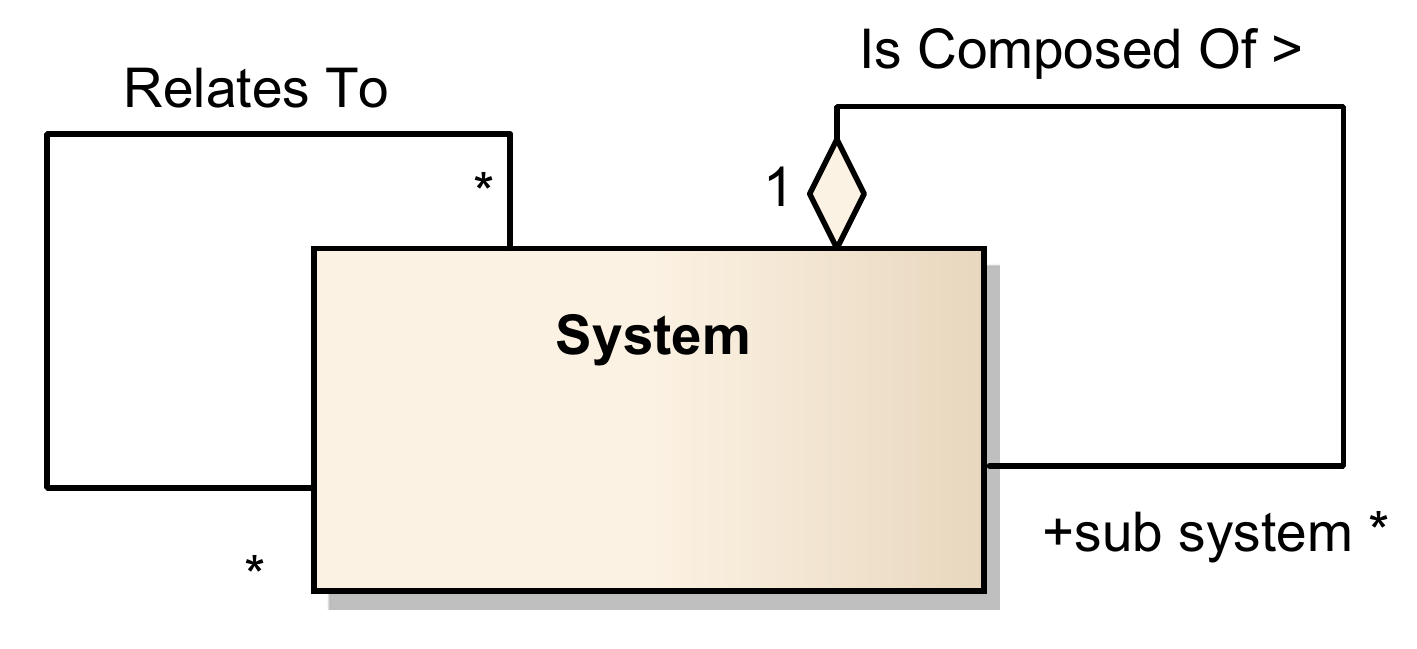
\includegraphics[width=0.6\textwidth]{./images/chapter3/system.png}
	\caption{Ορισμός του συστήματος.}
	\label{fig:system}
\end{figure}

\subsubsection{Μοντέλο}
\label{subsubsec:model}

Ένα \textit{Μοντέλο} είναι η απλουστευμένη αναπαράσταση ενός συστήματος, το οποίο μπορεί είτε να υφίσταται ήδη, είτε να δύναται να υφίσταται στο μέλλον. Το μοντέλο ορίζει το σύστημα και αντίστροφα. Ωστόσο, το μοντέλο από μόνο του είναι ένα σύστημα με δική του ταυτότητα, πολυπλοκότητα, χαρακτηριστικά, σχέσεις κ.τ.λ. Συνοψίζοντας, σύμφωνα και με το \ref{fig:model} μπορούμε να πούμε πως το μοντέλο είναι ένα σύστημα του οποίου ο σκοπός είναι ο καθορισμός ενός άλλου συστήματος, χωρίς να χρειάζεται να εξετάσουμε άμεσα το τελευταίο \cite{bib:rodrigues_2015}.

\begin{figure}[!ht]
	\centering
	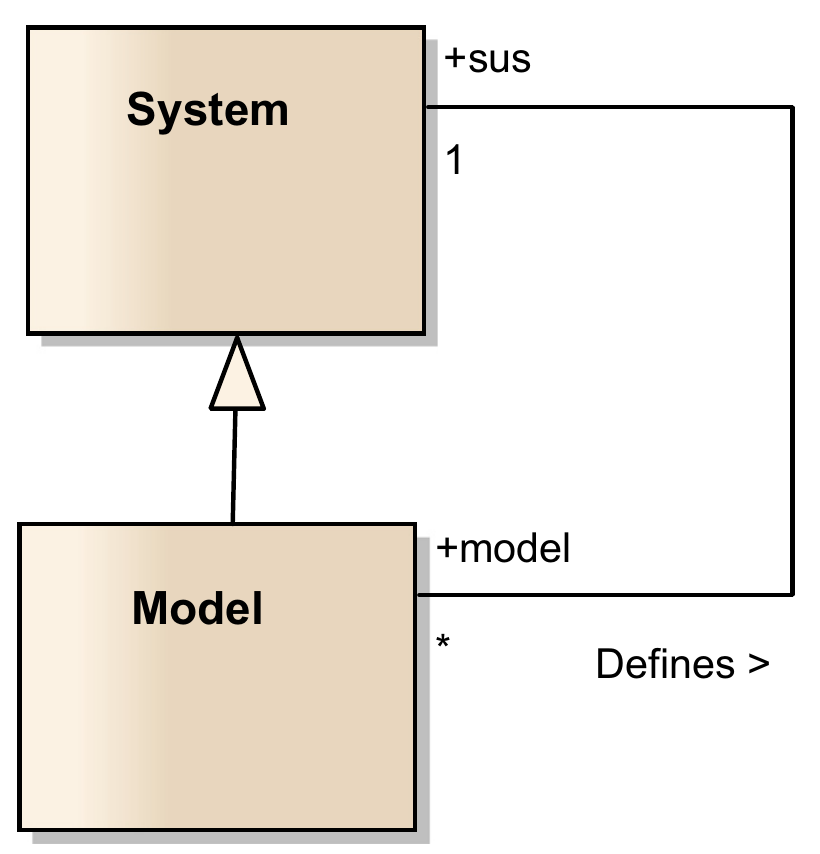
\includegraphics[width=0.4\textwidth]{./images/chapter3/model.png}
	\caption{Ορισμός του μοντέλου.}
	\label{fig:model}
\end{figure}

\subsubsection{Μετα-Μοντέλο}
\label{subsubsec:metamodel}

Όπως και για το μοντέλο, έτσι και για το \textit{Μετα-Μοντέλο}, δεν υπάρχει κάποιος κοινά αποδεκτός ορισμός. Θα μπορούσαμε ωστόσο να το χαρακτηρίσουμε ως μια απλουστευμένη αναπαράσταση ενός μοντέλου. Στην ουσία τα μετα-μοντέλα αποτελούν τον ορισμό μιας γλώσσας μοντελοποίησης, τον ορισμό της οποίας θα αναλύσουμε στη συνέχεια, καθώς παρέχουν έναν τρόπο περιγραφής όλων των μοντέλων που μπορούν να αναπαρασταθούν από τη συγκεκριμένη γλώσσα \cite{bib:brambilla_2012}. Μια αναπαράσταση του ορισμού του μετα-μοντέλου φαίνεται στο \autoref{fig:metamodel}.

\begin{figure}[!ht]
	\centering
	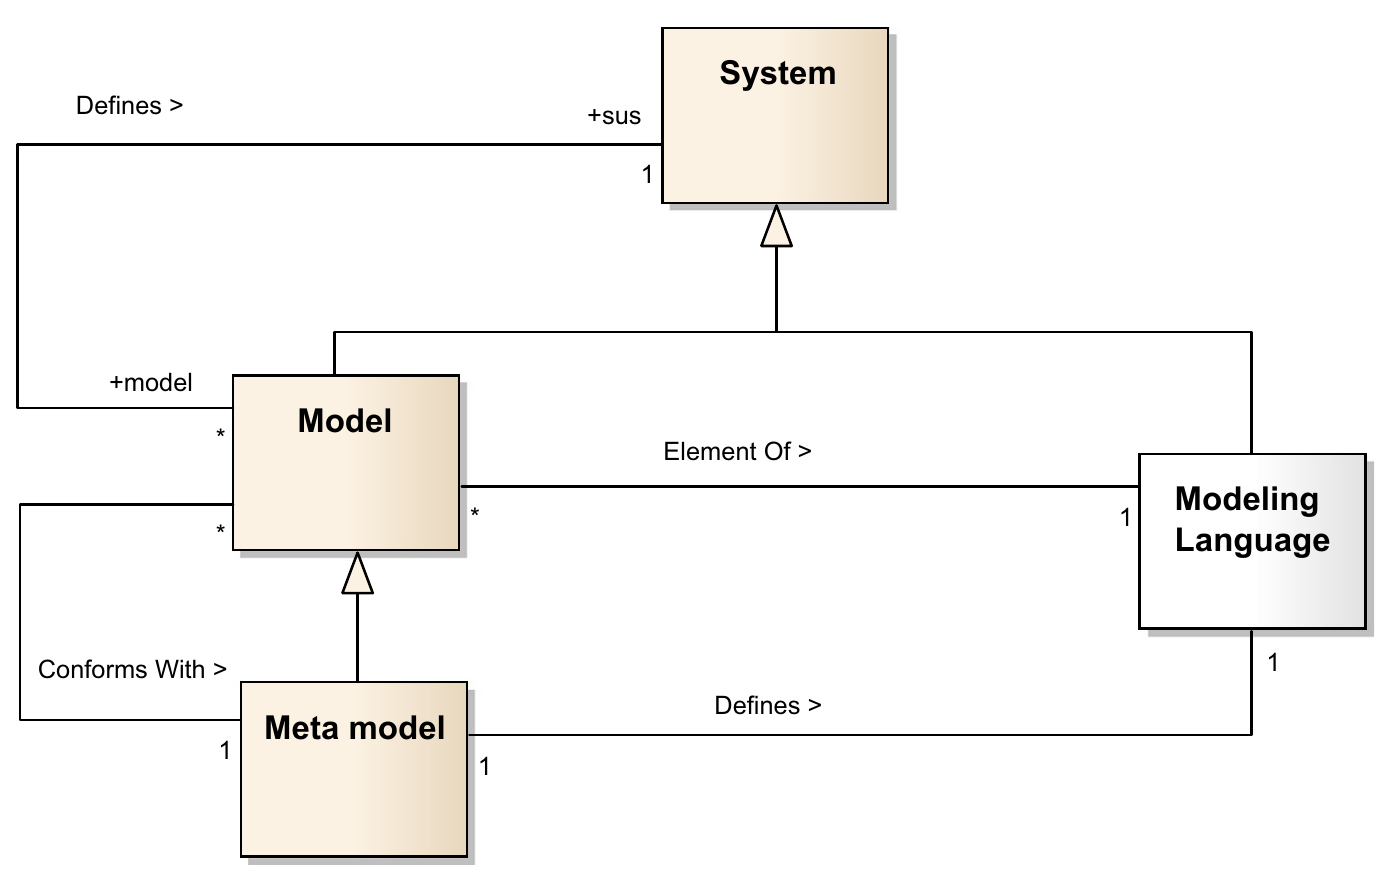
\includegraphics[width=1\textwidth]{./images/chapter3/metamodel.png}
	\caption{Ορισμός του μετα-μοντέλου.}
	\label{fig:metamodel}
\end{figure}

\subsection{Γλώσσες μοντελοποίησης}
\label{subsec:dsls}

Οι \textit{Γλώσσες Μοντελοποίησης} (\textit{Modeling Languages}) είναι ένα από τα βασικότερα κομμάτια της MDE. Μέσω αυτών γίνεται δυνατή η παρουσίαση ενός μοντέλου, και μπορεί να αποτελούνται είτε από γραφικές αναπαραστάσεις, είτε από προδιαγραφές μέσω κειμένου, είτε και από τα δύο. Οι γλώσσες αυτές χωρίζονται σε 2 μεγάλες κατηγορίες, τις γλώσσες συγκεκριμένου πεδίου και τις \textit{Γλώσσες Γενικού Σκοπού} (\textit{General Purpose Languages} ή \textit{GPL}). Μια DSL, είναι μία γλώσσα ειδικά σχεδιασμένη για έναν συγκεριμένο τομέα, σε αντίθεση με μία GPL, η οποία μπορεί να βρει εφαρμογή σε πληθώρα τομέων. Στο πλαίσιο της παρούσας εργασίας, αναπτύχθηκε μια DSL.

\subsection{Μετασχηματισμοί}
\label{subsec:transforms}

Πέρα από τα μοντέλα, οι \textit{Μετασχηματισμοί} που μπορούν να γίνουν στα μοντέλα είναι ένα ακόμα σημαντικό στοιχείο της MDE. Ένας μετασχηματισμός αποτελείται από ένα πλήθος κανόνων σύμφωνα με τους οποίους ένα μοντέλο εισοδου θα μετατραπεί σε ένα μοντέλο εξόδου. Υπάρχουν δύο είδη μεσασχηματισμών, οι οποίοι παρουσιάζονται παρακάτω.

\textit{\textbf{Μετασχηματισμός από μοντέλο σε μοντέλο (Model to Model transformation ή M2M)}}: Οι μετασχηματισμοί M2M γίνονται σύμφωνα με ένα σύνολο κανόνων, βάση των οποίων τα χαρακτηριστικά ενός μοντέλου μετατρέπονται σε χαρακτηριστικά ενός άλλου μοντέλου. Γίνεται δηλαδή μία \textit{αντιστοίχηση των στοιχείων} τους (\textit{model mapping}).

\textit{\textbf{Μετασχηματισμός από μοντέλο σε κώδικα (Model to Text transformation ή M2T)}}: Κατά τη διαδικασία αυτή, σύμφωνα πάλι με ένα σύνολο κανόνων, από τα στοιχεία του μοντέλου παράγεται κώδικας προς εκτέλεση, με βάση κάποια συγκεκριμένα πρότυπα.